\documentclass[t]{beamer}
\usetheme[height=7mm]{Rochester}
\setbeamercovered{transparent}
\setbeamertemplate{navigation symbols}{}
%\setbeamertemplate{footline}[frame number]
\setbeamertemplate{footline}
{
\leavevmode%
  \hbox{%
  \begin{beamercolorbox}[wd=\paperwidth,dp=2.5ex,ht=3ex]{}%
    \hspace*{2em}%
    {\hfill Folie \insertframenumber}%
    \hspace*{2em}%
  \end{beamercolorbox}%
  }%
}

\usepackage[german]{babel}
\usepackage[utf8]{inputenc}
\usepackage[vlined]{algorithm2e}
\DontPrintSemicolon

\theoremstyle{plain}
\newtheorem{Korollar}{Korollar}


\title[Treaps]{Randomisierte Suchstrukturen: Treaps}
\author[M. Beck, R. McDaniel]{Moritz Beck, Robert McDaniel}
\date[10.06.2015]{10. Juni 2015}


\AtBeginSection[]{
    {\setbeamertemplate{footline}{}
    \begin{frame}<beamer>{Gliederung}
        \tableofcontents[currentsection]
    \end{frame}}
}
\AtBeginSubsection[]{
    {\setbeamertemplate{footline}{}
    \begin{frame}<beamer>{Gliederung}
        \tableofcontents[currentsubsection]
    \end{frame}}
}

\beamerdefaultoverlayspecification{<+->}

\begin{document}

{
\setbeamertemplate{footline}{}

\begin{frame}%[plain]
    \titlepage
\end{frame}

\begin{frame}{Gliederung}
    \tableofcontents
\end{frame}
}

\section{Einführung und Motivation}
\subsection{Grundmotivation}
\begin{frame}{Grundmotivation}
    Gesucht: Möglichst schnelle Datenstruktur mit Unterstützung folgender Methoden:
    \bigskip
    \begin{itemize}
        \item<2-> $S$ = MakeSet()
        \item<3-> Insert($i, S$)
        \item<4-> Delete($k, S$)
        \item<5-> Find($k, S$)
        \item<6-> $S$ = Join$(S_1, i, S_2)$
        \item<7-> $S$ = Paste$(S_1, S_2)$
        \item<8-> $S_1, S_2$ = Split$(k, S)$ 
    \end{itemize}
    \bigskip
    \onslide<9-> Bereits bekannt: Binäre Suchbäume
\end{frame}

\subsection{Laufzeiten bei binären Suchbäumen}
\begin{frame}{Laufzeiten bei binären Suchbäumen}
    \setbeamercovered{invisible}
    $h$ = Höhe des Baums
    \begin{table}
        \begin{tabular}{l | c }
        Methode & Laufzeit\\
        \hline % TODO: Tabellenstruktur vorher schon anzeigen (wie in Zeile 1 oder 2)
        \only<2->{$S$ = MakeSet()} & \only<2->{$O(1)$}\\
        \visible<3->{Insert$(i, S)$} & \visible<3->{$O(h)$} \\
        \onslide<4-> Delete$(k, S)$ & $O(h)$ \\
        \onslide<5-> Find$(k, S)$ & $O(h)$ \\
        \onslide<6-> $S$ = Join($S_1, i, S_2$) & STUFF \\
        \onslide<7-> $S$ = Paste($S_1, S_2$) & STUFF \\
        \onslide<8-> $S_1, S_2$ = Split$(k, S)$ & STUFF 
        %TODO: Laufzeiten für Join/Paste/Split? -> steht indirekt im Buch (Implementierung)
        % TODO: geht die Tabelle auch größer? das sieht irgendwie komisch aus
        \end{tabular}
    \end{table}
\end{frame}

\subsection{Probleme bei binären Suchbäumen}
    \begin{frame}{Probleme bei binären Suchbäumen}
    \begin{itemize}
    \item Es zeichnet sich ab: Hohe Abhängigkeit von Höhe des Baums $\Rightarrow$ Schwanken zwischen $O(\log(n))$ und $O(n)$
    \item Problem: Binärbäume sind oft unoptimal und extreme Fälle führen zu langen Laufzeiten!
    \end{itemize}
    {\only<3->{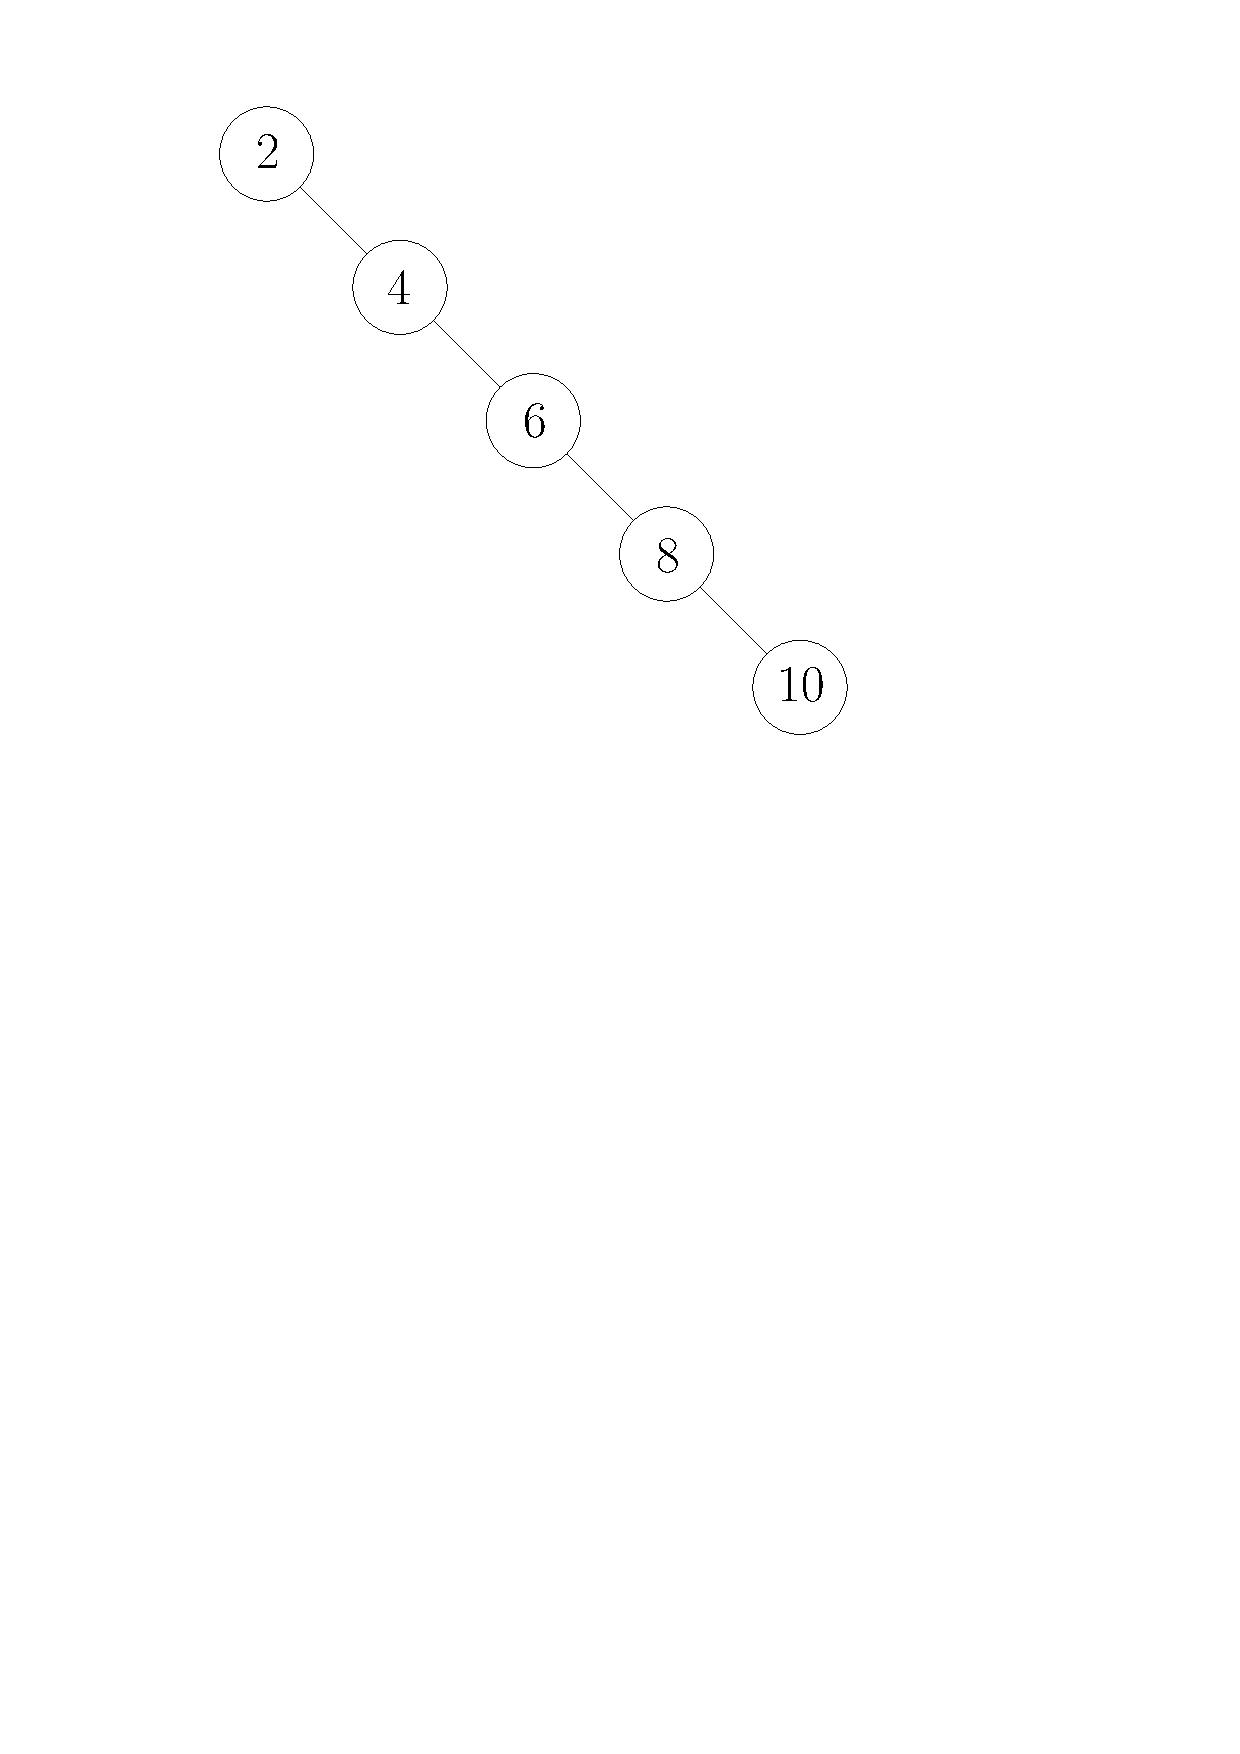
\includegraphics[width=.5\textwidth] {img/BinaryTree.pdf}}}
    % TODO: Centering? -> würde ich schon machen
\end{frame}

\begin{frame}{Probleme bei binären Suchbäumen}
    \begin{itemize}
    \item Problem: Hohe worst-case-Laufzeiten
    \item Lösung: Vorherige Optimierung (Balancieren)?
    \item Implementierung von Balancieren bringt neue Probleme:
        \begin{itemize}
        \item Erhöhter Overhead
        \item Höhere Laufzeiten durch konstantes Updating
        \item Speichern von zusätzlicher Information möglicherweise notwendig
        \end{itemize}
    \bigskip
    \item Lösungsidee: Balancieren durch Randomisieren?
    \begin{itemize}
        \item Einfache Implementierung
        \item Keine weitere Information zu speichern
        \item Schnelle Ausführung
    \end{itemize}
\end{itemize}
\end{frame}


\section{Treaps}
\subsection{Grundlagen}
\begin{frame}{Titel}
    \begin{center}
        \color{red}{Binary \textbf{Tr}ee} + \color{blue}{H\textbf{eap}} = \textbf{\textcolor{red}{Tr}\textcolor{blue}{eap}}
    \end{center}
    \begin{itemize}
        \item<2-> \textcolor{red}{Schlüssel}
        \item<3-> \textcolor{blue}{Priorität} (meist Implementierungsdetail)
    \end{itemize}
    \vspace{1em}
    \hfill\only<4->{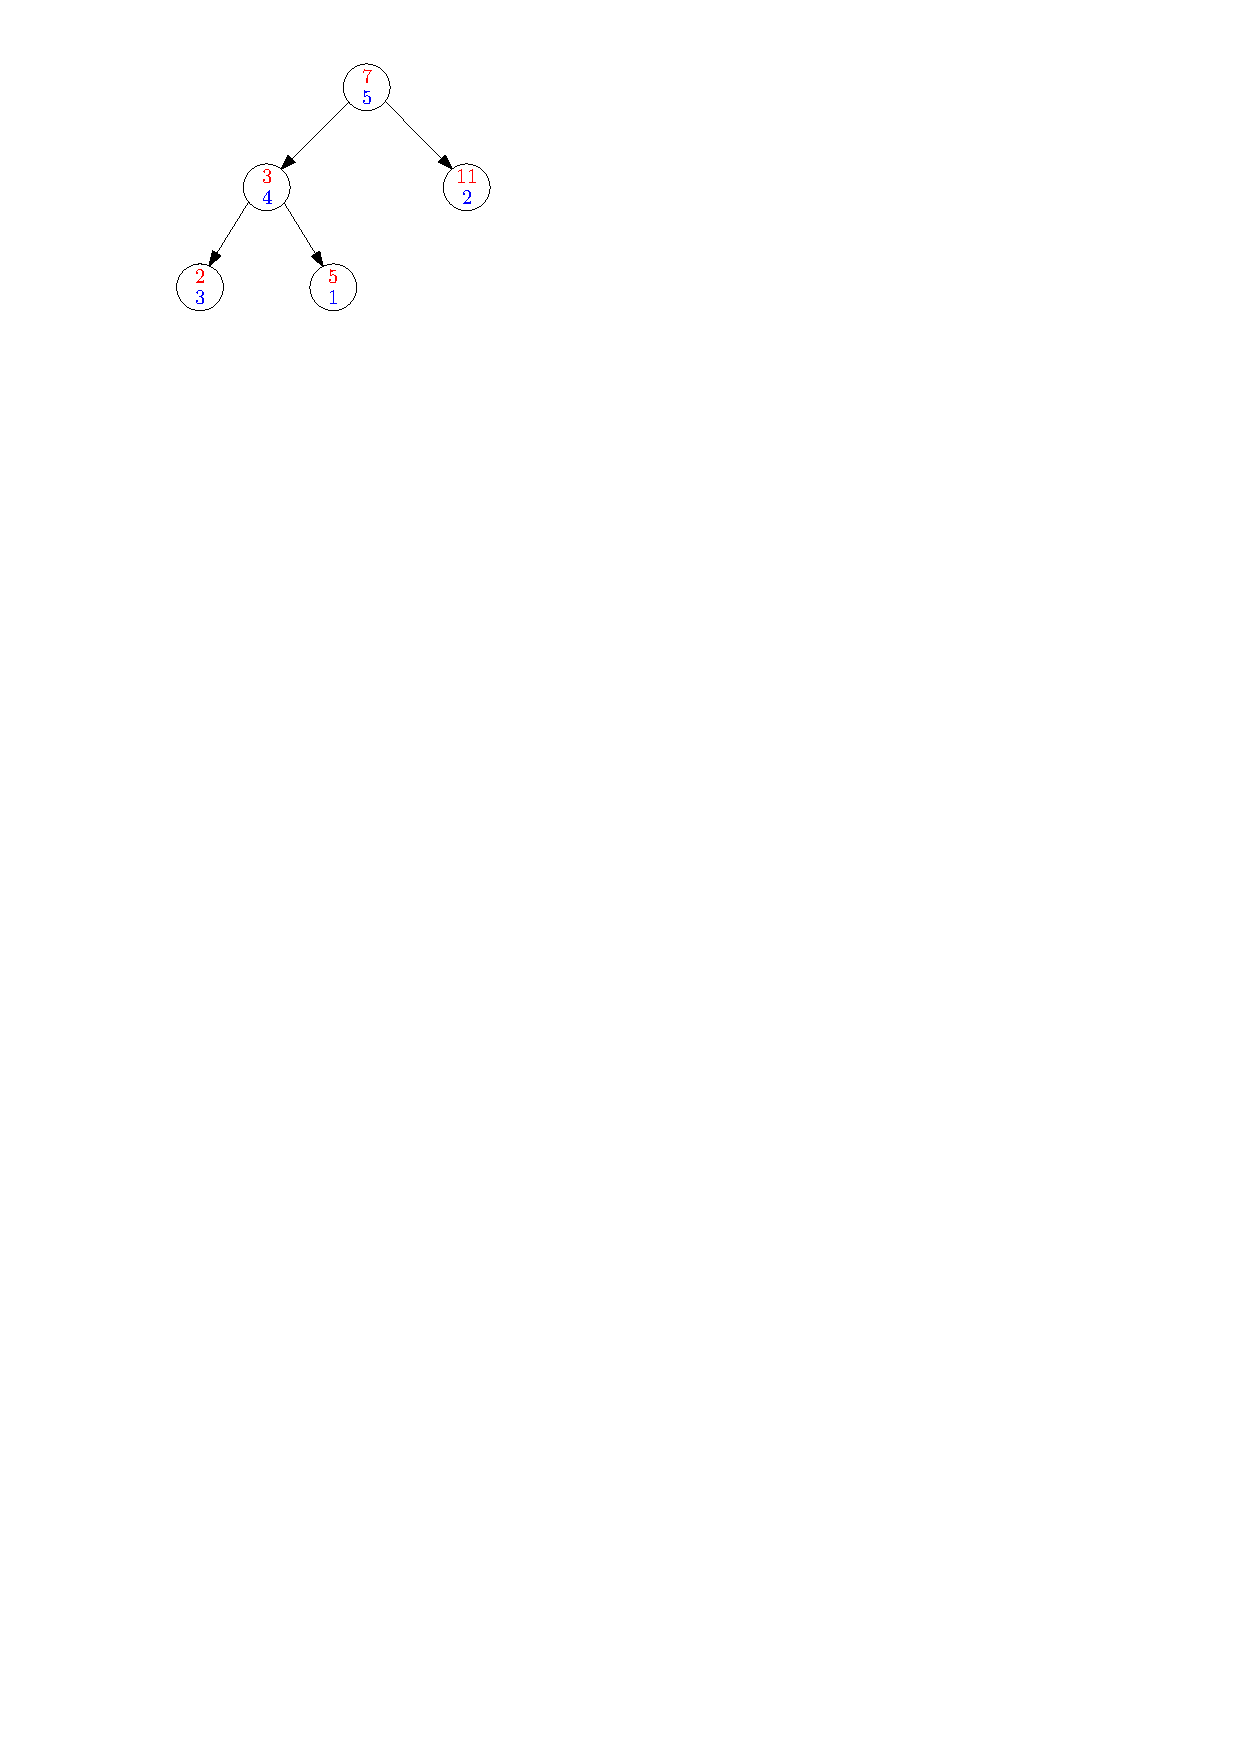
\includegraphics[page=1,width=.5\textwidth]{img/Beispiel_Treap.pdf}}
\end{frame}

\subsection{Existenz eindeutiger Treaps}
\begin{frame}{Titel}
    \begin{Satz}
        Für jede Menge $S = \{(k_1,p_1), \dots, (k_n, p_n)\}$ von Schlüssel-Priorität-Paaren mit paarweise unterschiedlichen Schlüsseln und Prioritäten existiert genau ein gültiger Treap.
    \end{Satz}
    \only<2-5>{
    \begin{proof}
        Per Induktion über $n = \left|S\right|$:
        \raisebox{3em}{
        \begin{columns}<2->
        \begin{column}[t]{.65\textwidth}
            \begin{itemize}
            \item<3-> \textbf{IA}: n = 0: \\ leere Menge $\leftrightarrow$ leerer Baum \textcolor[rgb]{0,.7,0}{\Large\checkmark}
            \item<4-> \textbf{IS}: $t   = \{(k_t, p_t) \in S \mid p_t \text{ minimal}\}$
                                   $M_< = \{(k_i, p_i) \in S \mid k_i < k_t\}$ \\
                                   $M_> = \{(k_i, p_i) \in S \mid k_i > k_t\}$
            \end{itemize}
        \end{column}
        \begin{column}[t]{0.35\textwidth}
            \raisebox{-\totalheight}{\visible<5->{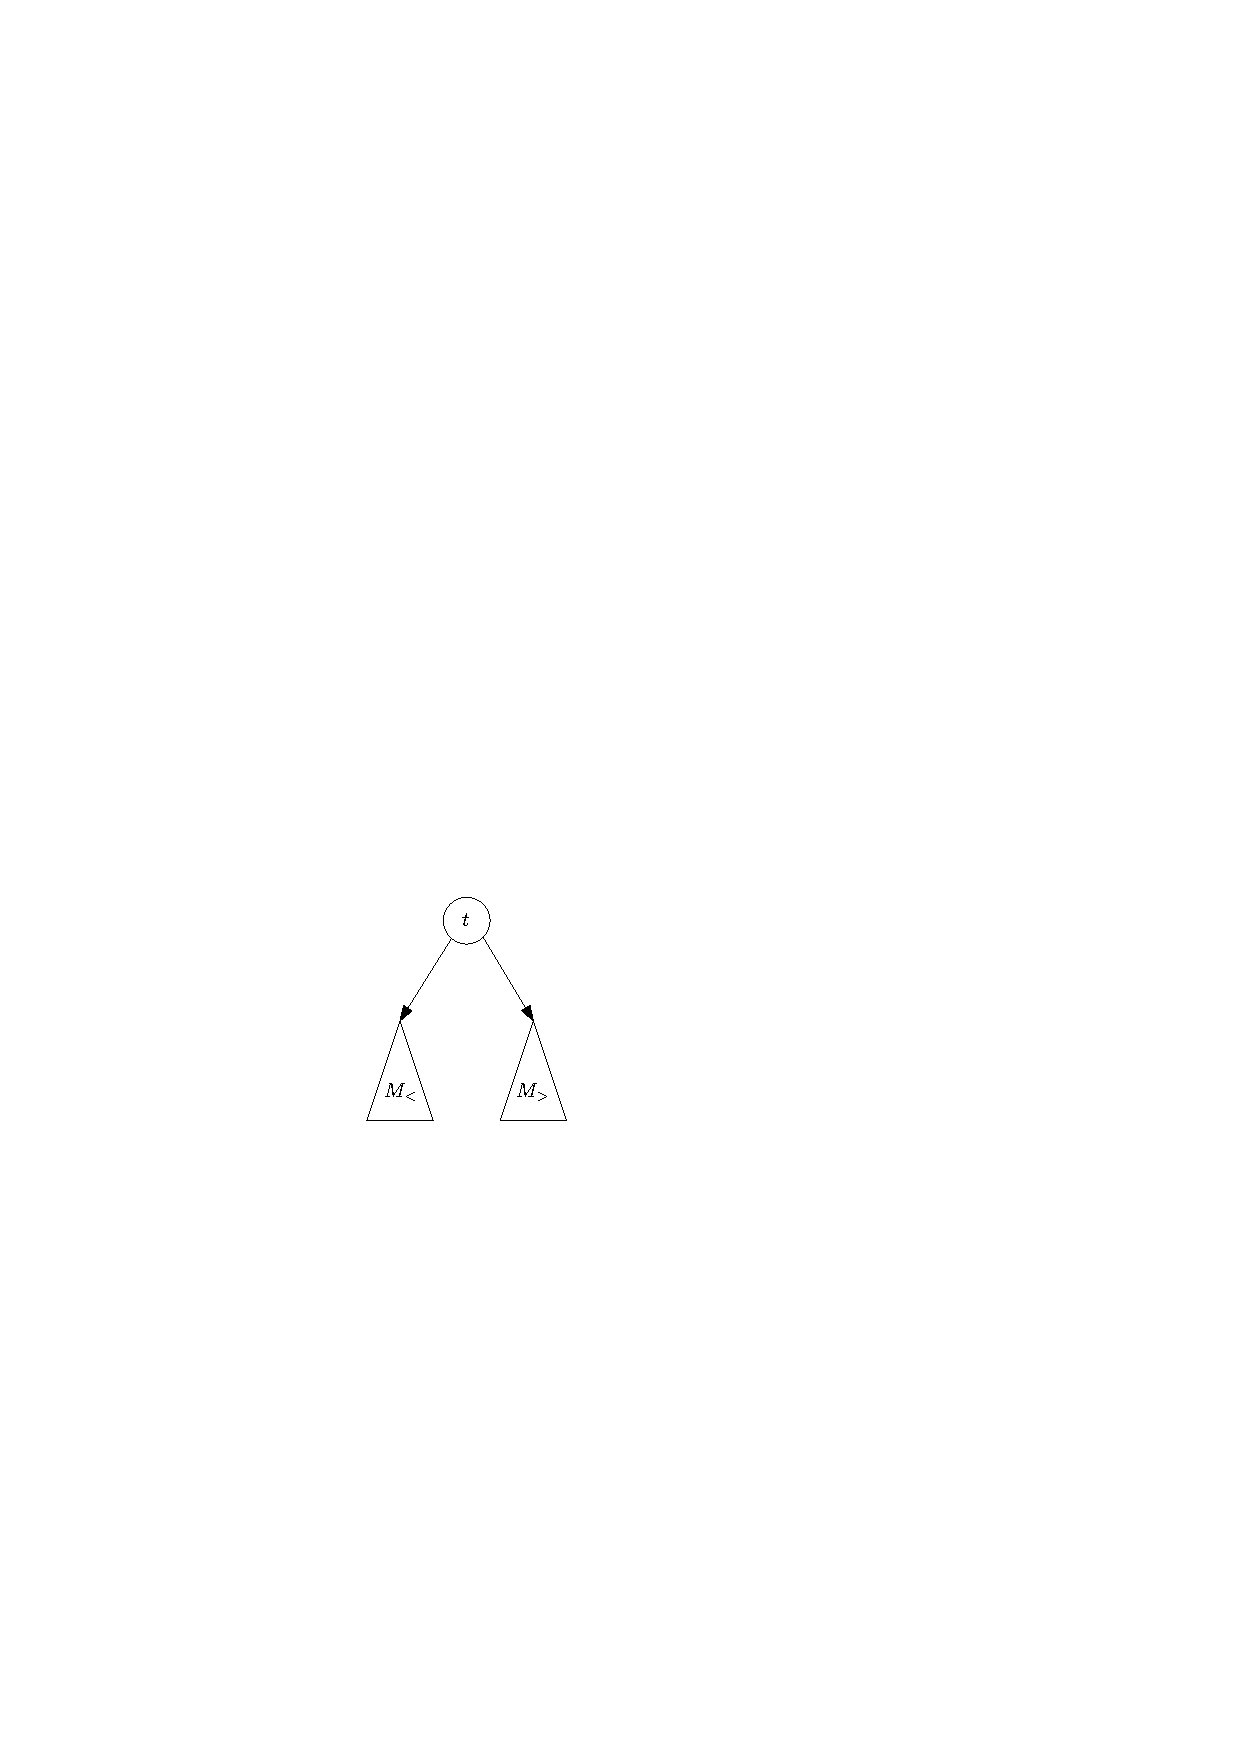
\includegraphics[width=.9\textwidth]{img/Eindeutigkeit_IS.pdf}}}
        \end{column}
        \end{columns}}
    \end{proof}}
    \visible<6->{\begin{Folgerung}
        Die Reihenfolge, in der Knoten eingefügt oder gelöscht werden, ist für die Struktur eines Treaps irrelevant.
    \end{Folgerung}}
\end{frame}

\subsection{Implementierung}
% TODO: Folie für Rotation
\begin{frame}{Titel}
    \begin{columns}<1->
    \begin{column}{.65\textwidth}<1->
        \begin{itemize}
            \item<1> Find($k$, $S$): Normale Suche in einem Binärbaum
            \item<2> Insert($i$, $S$):
                \begin{algorithm}[H]
                    %\Ein{Knoten $i$, Treap $S$}
                    Füge $i$ als Blatt in $S$ ein \;
                    \While{$i$.parent.prio $<$ $i$.prio}{
                        Rotiere $i$ nach oben \;
                    }
                \end{algorithm}
            \item<3> Delete($i$, $S$):
                \begin{algorithm}[H]
                    \SetKw{Not}{not}
                    \While{\Not istBlatt($i$)}{
                        Rotiere $i$ nach unten \;
                    }
                    Lösche Blatt $i$ aus $S$ \;
                \end{algorithm}
        \end{itemize}
    \end{column}
    \begin{column}{.35\textwidth}<1->
        \raisebox{-\totalheight}{
            %\only<1>{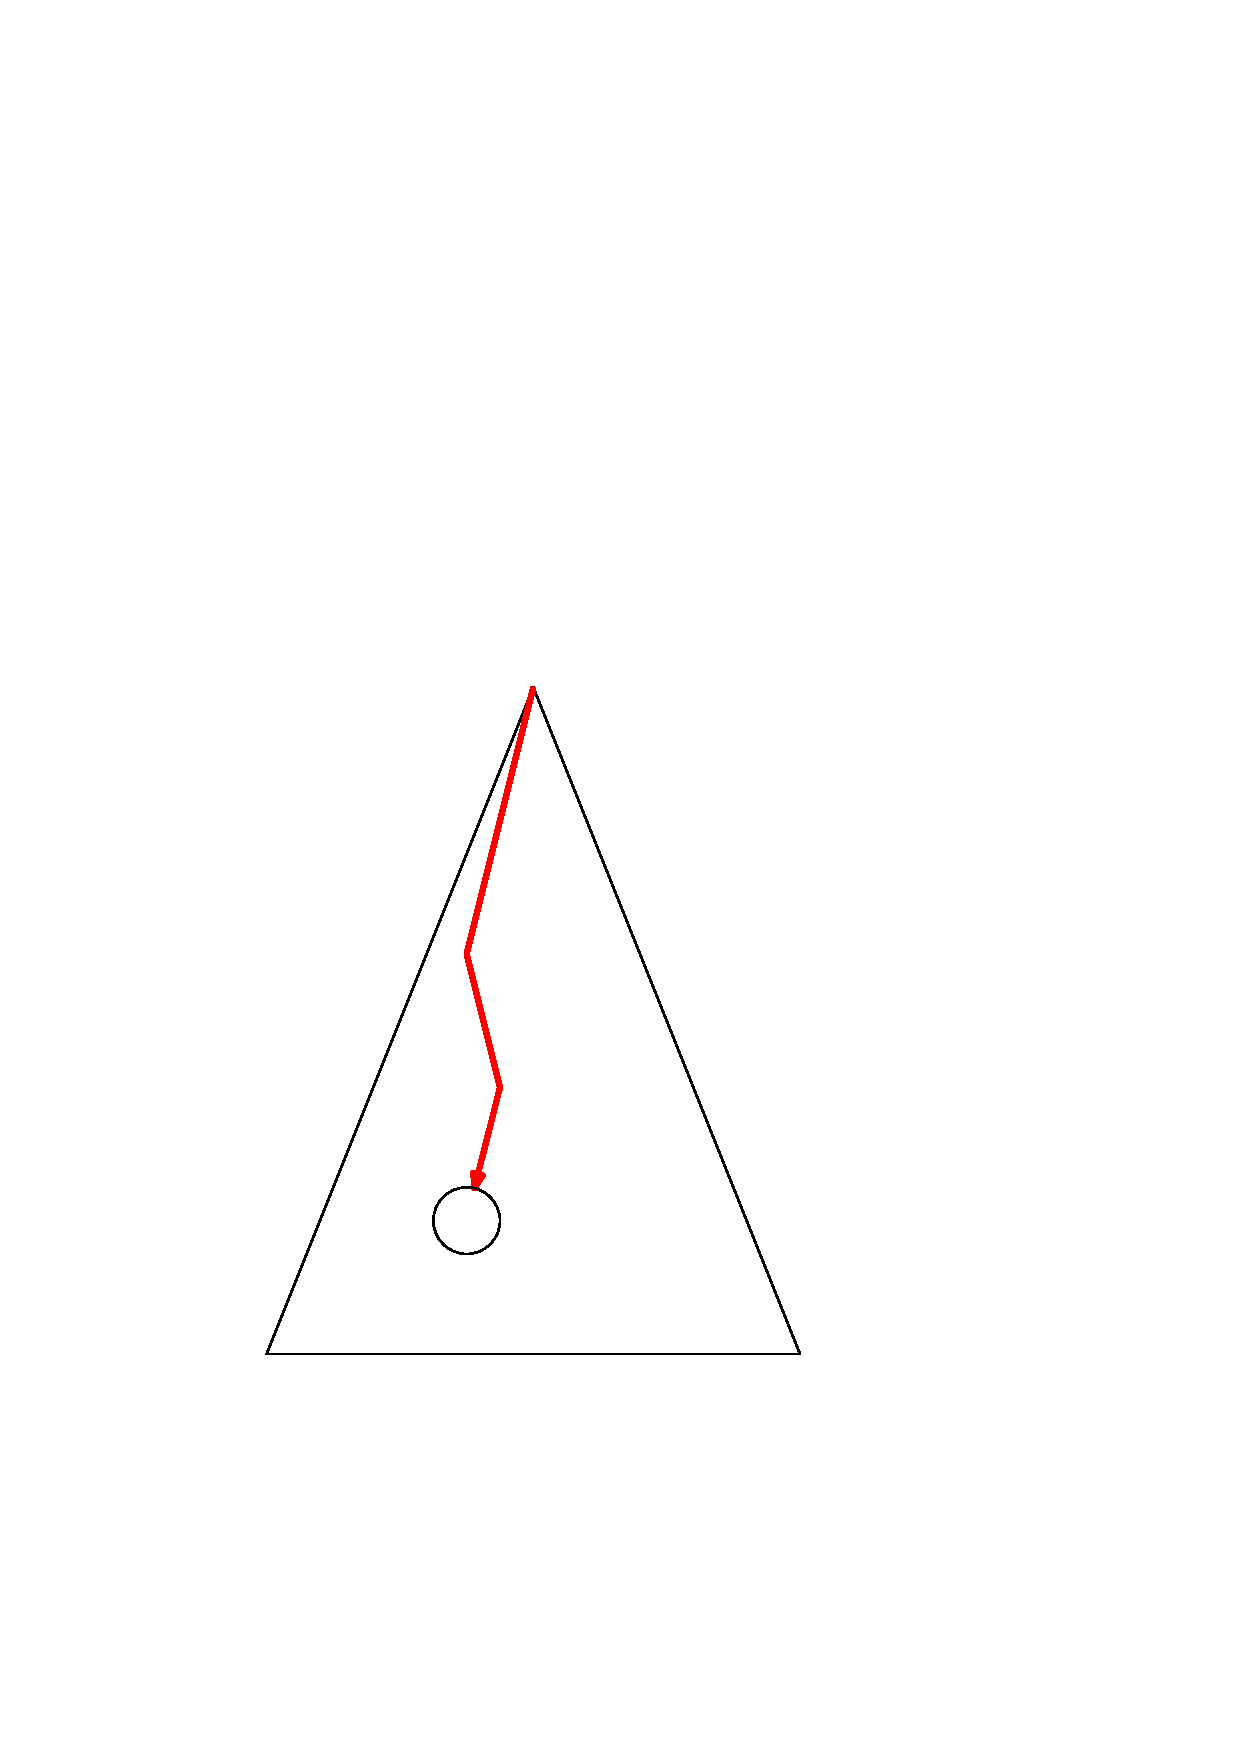
\includegraphics[width=.8\textwidth]{img/Impl_Find.pdf}} %TODO: Bild fehlt noch
            %\only<2>{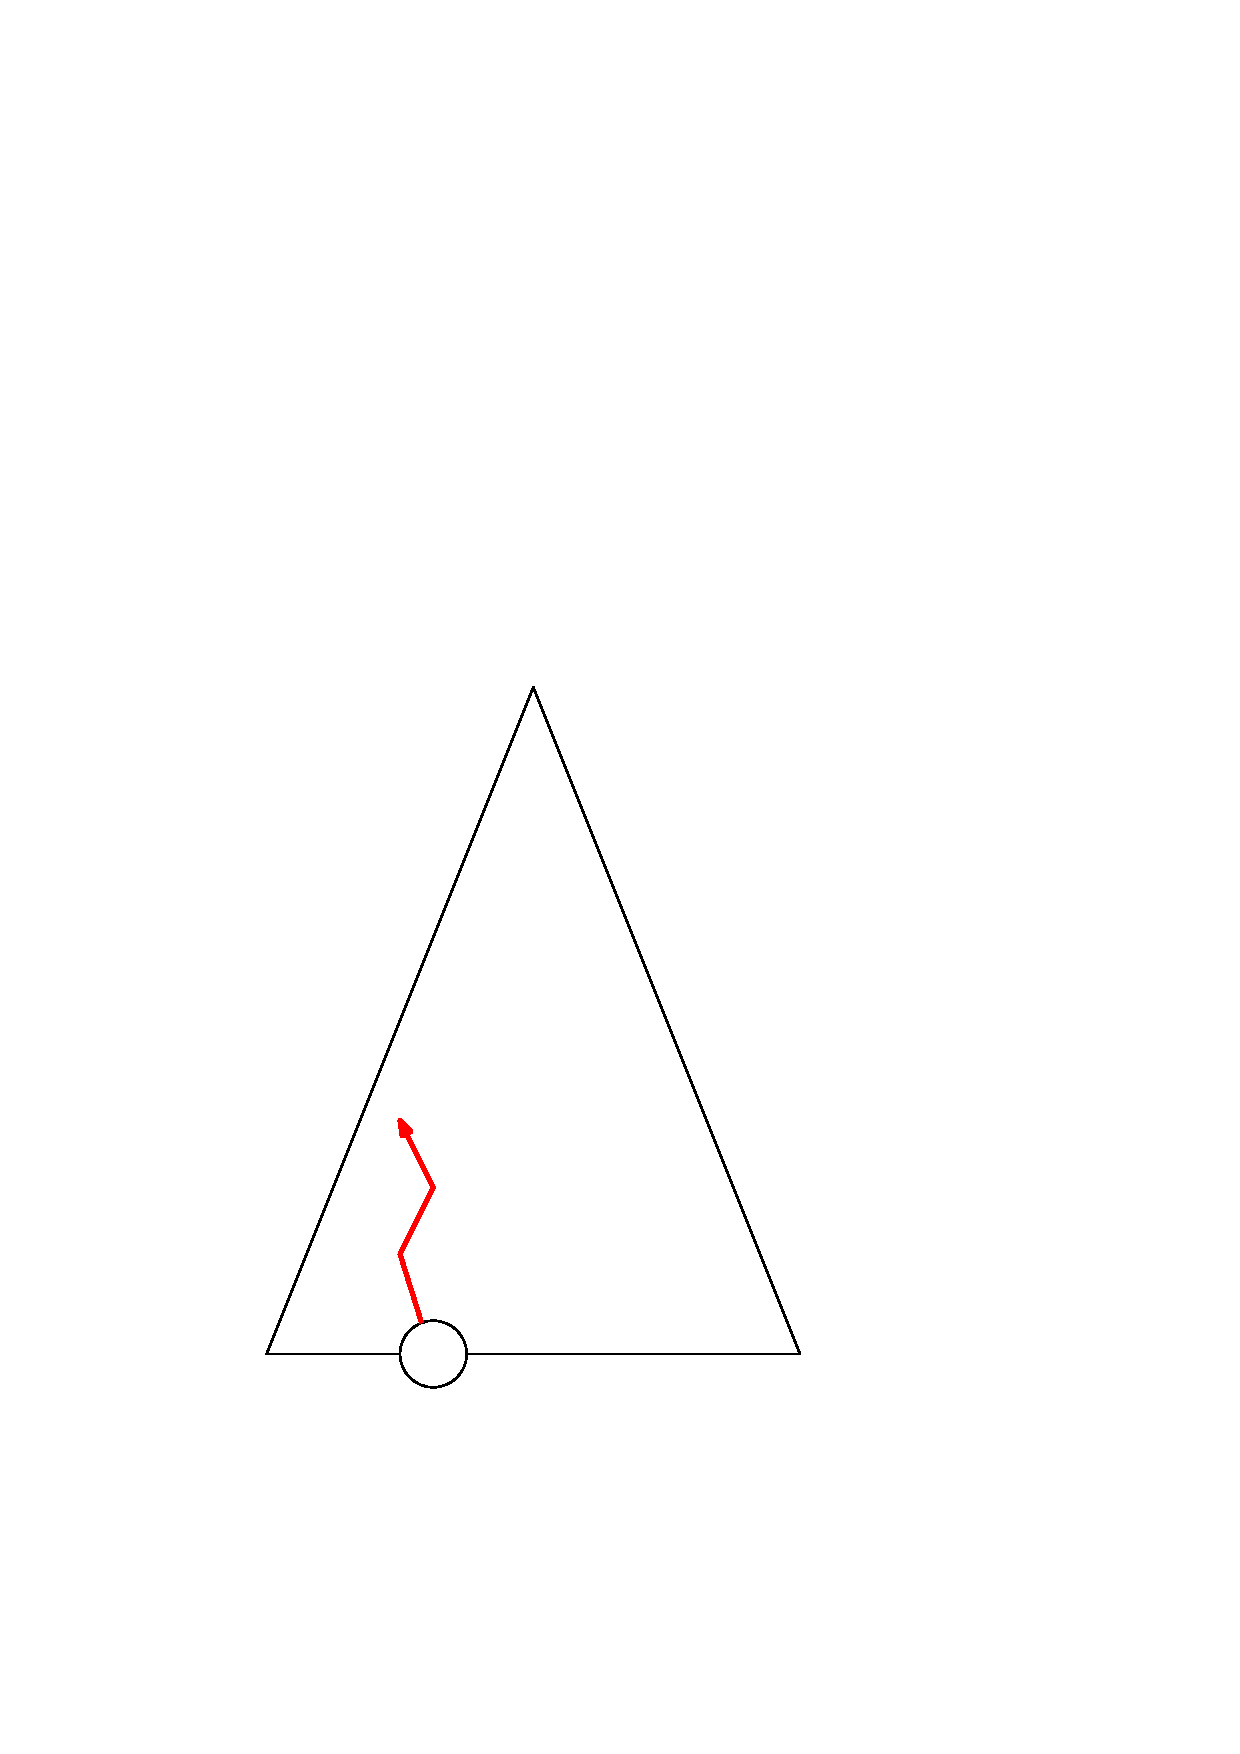
\includegraphics[width=.8\textwidth]{img/Impl_Insert.pdf}} %TODO: Bild fehlt noch
            %\only<3>{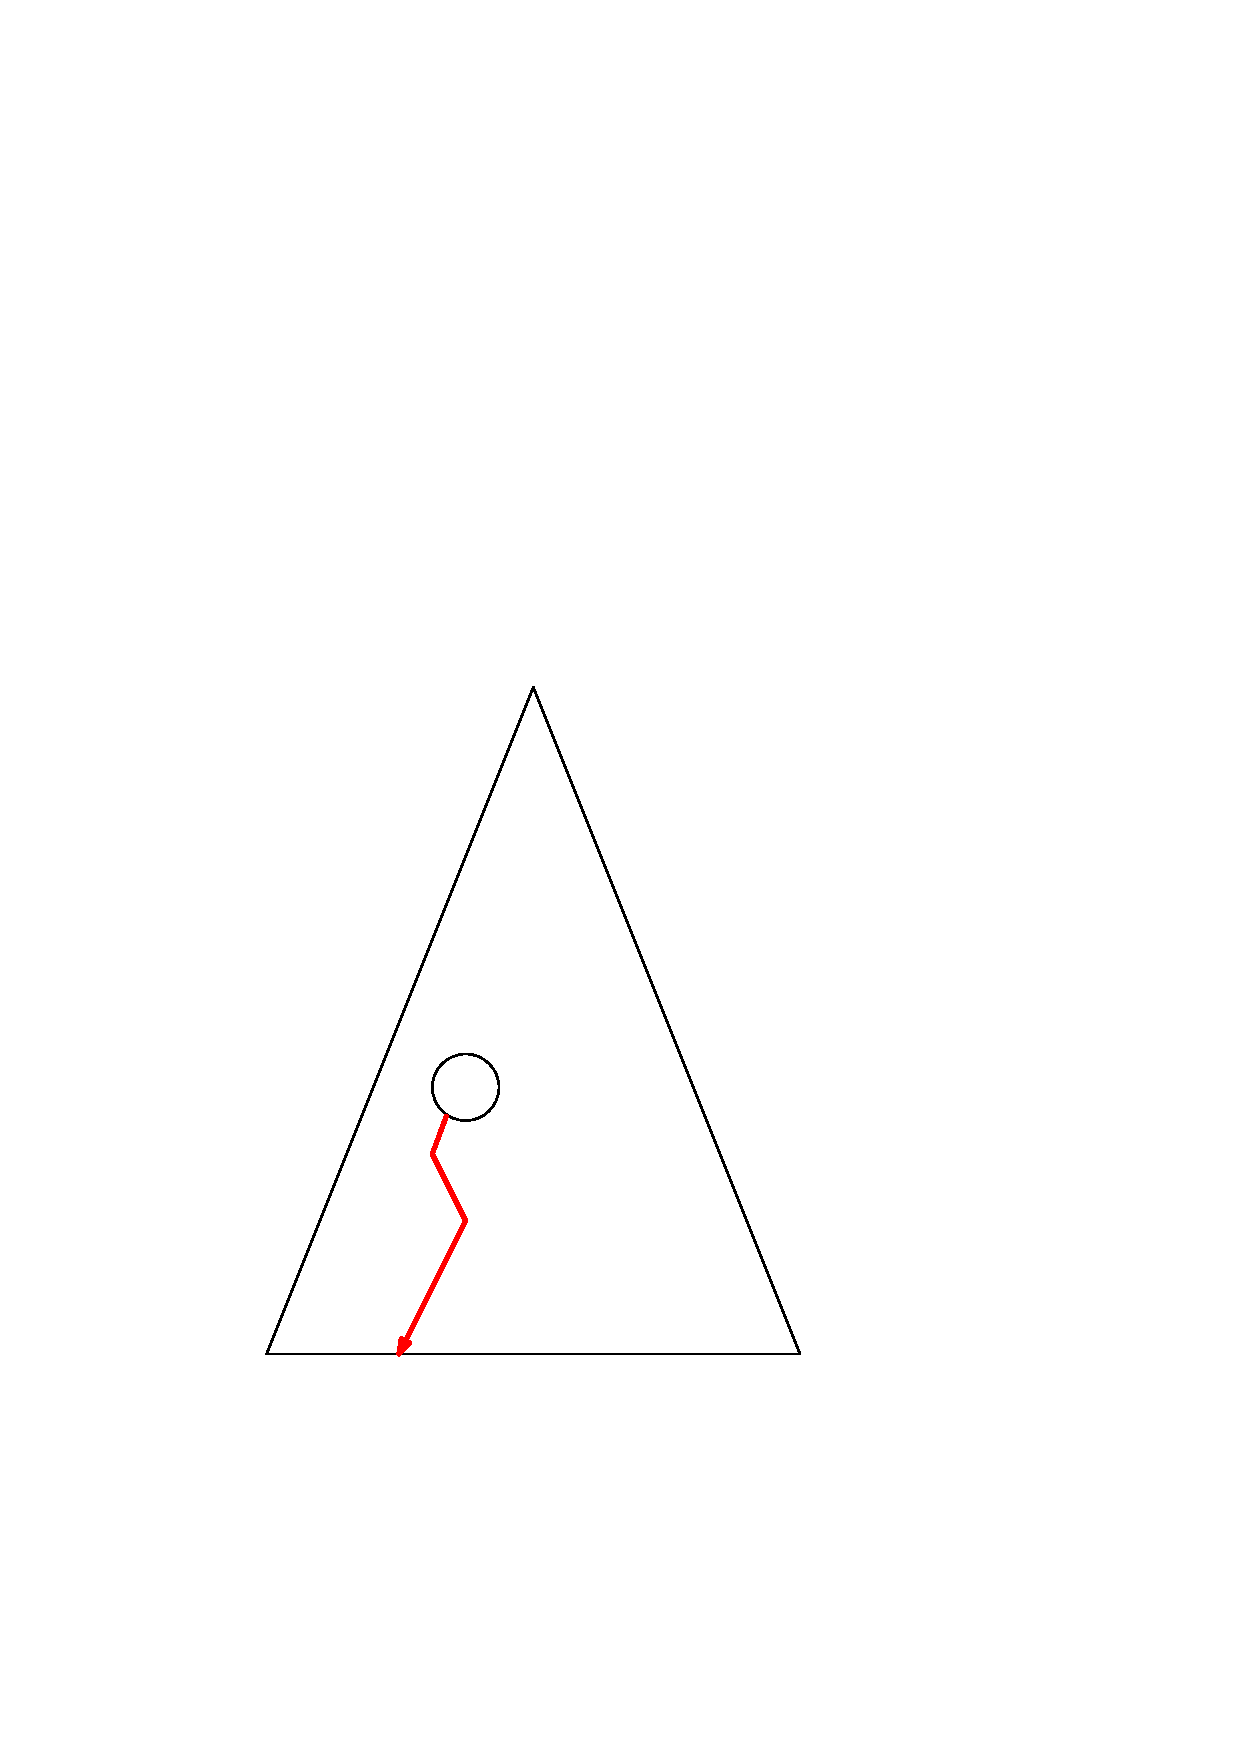
\includegraphics[width=.8\textwidth]{img/Impl_Delete.pdf}} %TODO: Bild fehlt noch
        }
    \end{column}
    \end{columns}
% Insert(i, S) // S wird verändert
% Delete(k, S) // S wird verändert
% Find(k, S)
% S = Join(S_1, i, S_2)
% S = Paste(S_1, S_2)
% S_1, S_2 = Split(k, S)
\end{frame}

\begin{frame}{Titel}
    \begin{columns}<1->
    \begin{column}{.65\textwidth}<1->
        \begin{itemize}
            \item<1> Join($S_1$, $i$, $S_2$):
                \begin{algorithm}[H]
                    \SetKw{Or}{or}
                    $i$.left $\gets S_1$ \;
                    $i$.right $\gets S_2$ \;
                    \While{$i$.prio $<$ $i$.left.prio\\ \Or $i$.prio $<$ $i$.right.prio}{
                        Rotiere $i$ nach unten \;
                    }
                    \Return $i$
                \end{algorithm}
            \item<2> Paste($S_1$, $S_2$):
                \begin{algorithm}[H]
                    $i$ $\gets$ Find($\infty$, $S_1$) \tcp{Maximum}
                    Delete($i$, $S_1$) \;
                    \Return Join($S_1$, $i$, $S_2$) \;
                \end{algorithm}
            \item<3> Split($k$, $S$):
                \begin{algorithm}[H]
                % TODO?
                    \tcp{Übungsaufgabe ;-)}
                \end{algorithm}
        \end{itemize}
    \end{column}
    \begin{column}{.35\textwidth}<1->
        \raisebox{-\totalheight}{
            %\only<1>{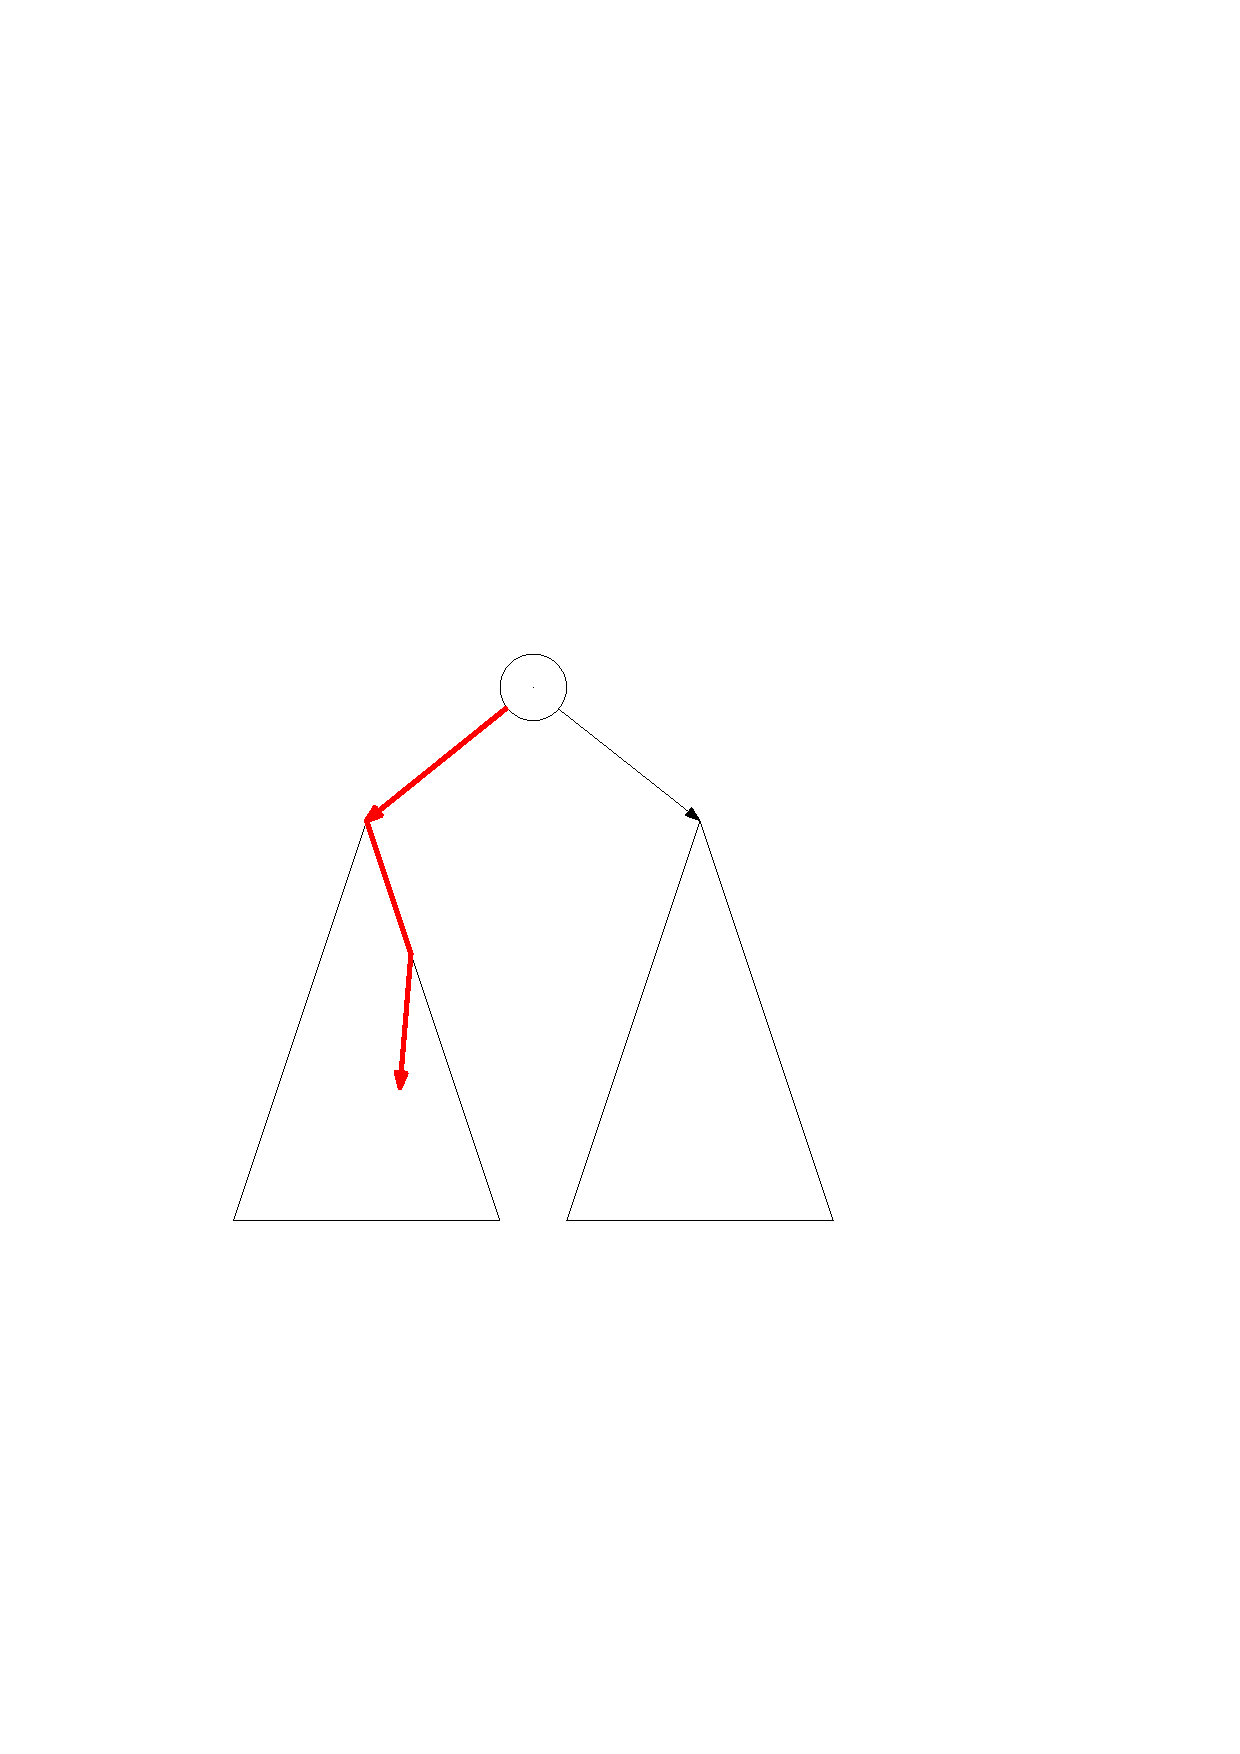
\includegraphics[width=.8\textwidth]{img/Impl_Join.pdf}} %TODO: Bild fehlt noch
            %\only<2>{\includegraphics[width=.8\textwidth]{img/Impl_Paste.pdf}} %TODO: Bild fehlt noch
            %\only<3>{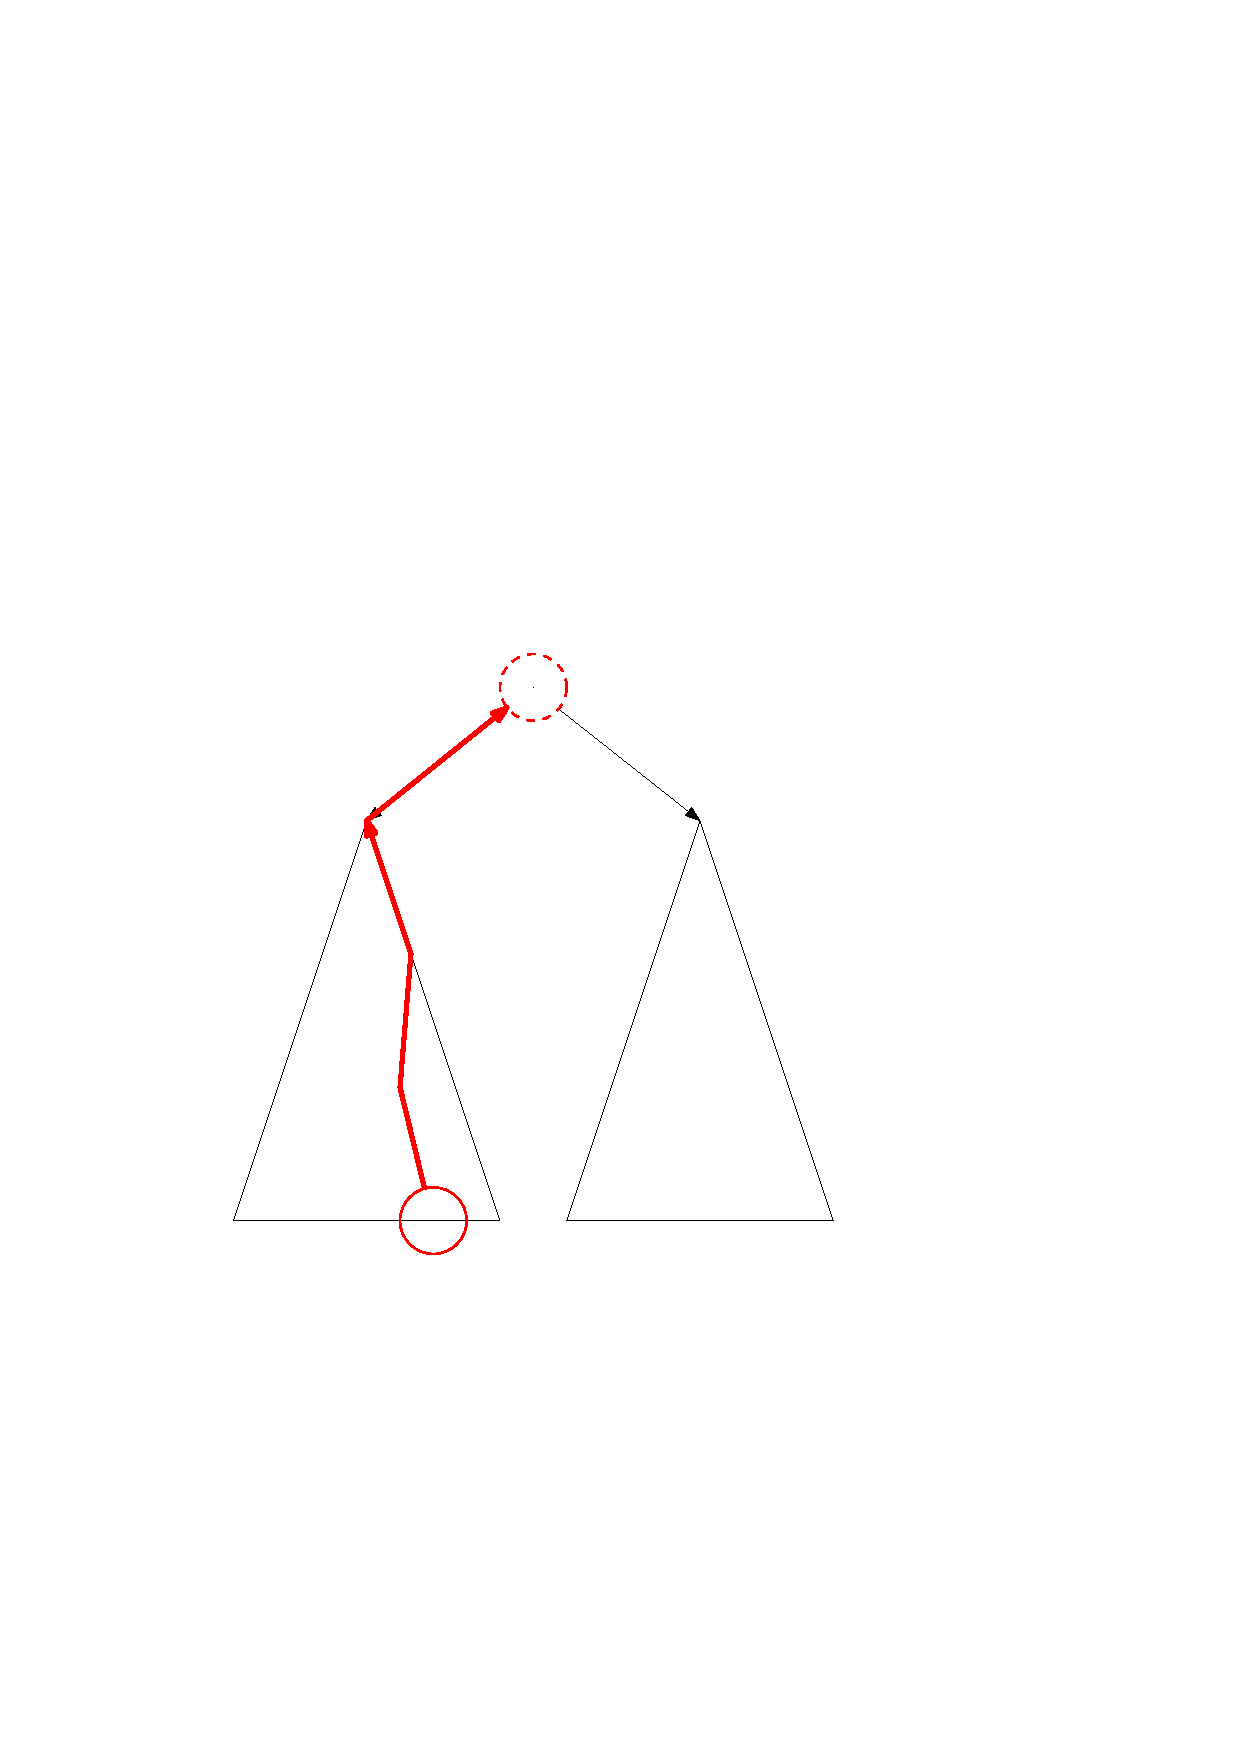
\includegraphics[width=.8\textwidth]{img/Impl_Split.pdf}} %TODO: Bild fehlt noch
        }
    \end{column}
    \end{columns}
% Insert(i, S) // S wird verändert
% Delete(k, S) // S wird verändert
% Find(k, S)
% S = Join(S_1, i, S_2)
% S = Paste(S_1, S_2)
% S_1, S_2 = Split(k, S)
\end{frame}

\subsection{Laufzeitanalyse}
\begin{frame}{Titel}
    
\end{frame}


\section*{Fazit}
\begin{frame}{Fazit}
    
\end{frame}



% \section{Skip-Lists}
% \subsection{Grundlagen}
% \begin{frame}{Titel}
    
% \end{frame}

% \section*{Ende}
% {\setbeamertemplate{footline}{}
% \begin{frame}<beamer>[c]
    % \begin{center}
    % \Huge{Fragen?}
    % \end{center}
% \end{frame}}

\end{document}